\chapter{变压器}
\begin{wrapfigure}[7]{r}{0.15\textwidth}
    \centering
    
\includegraphics[width=0.15\textwidth]{恩里克·普奇.png}
    \caption{时间要加速了!}
\end{wrapfigure}
\Par 好了,到了变压器,我们就可以“稍微”加快一点进度了,接下来讲的东西会比较的快和浅,因此具体的原理可能不会讲,只讲一下表面的现象规律,不要介意,这是这门课的特点,学时不够嘛.

\Par 变压器这一节也就讲一点东西,所以我们这里也就不搞什么章前的内容提要了.

\Par 如图\ref{fig:变压器原理图}所示即为变压器的基本结构,左边的绕线组与电源相连,我们称之为\textbf{一次绕组};右边的绕线组与负载相连,我们称之为\textbf{二次绕组}.
\begin{figure}[htbp]
	\centering
	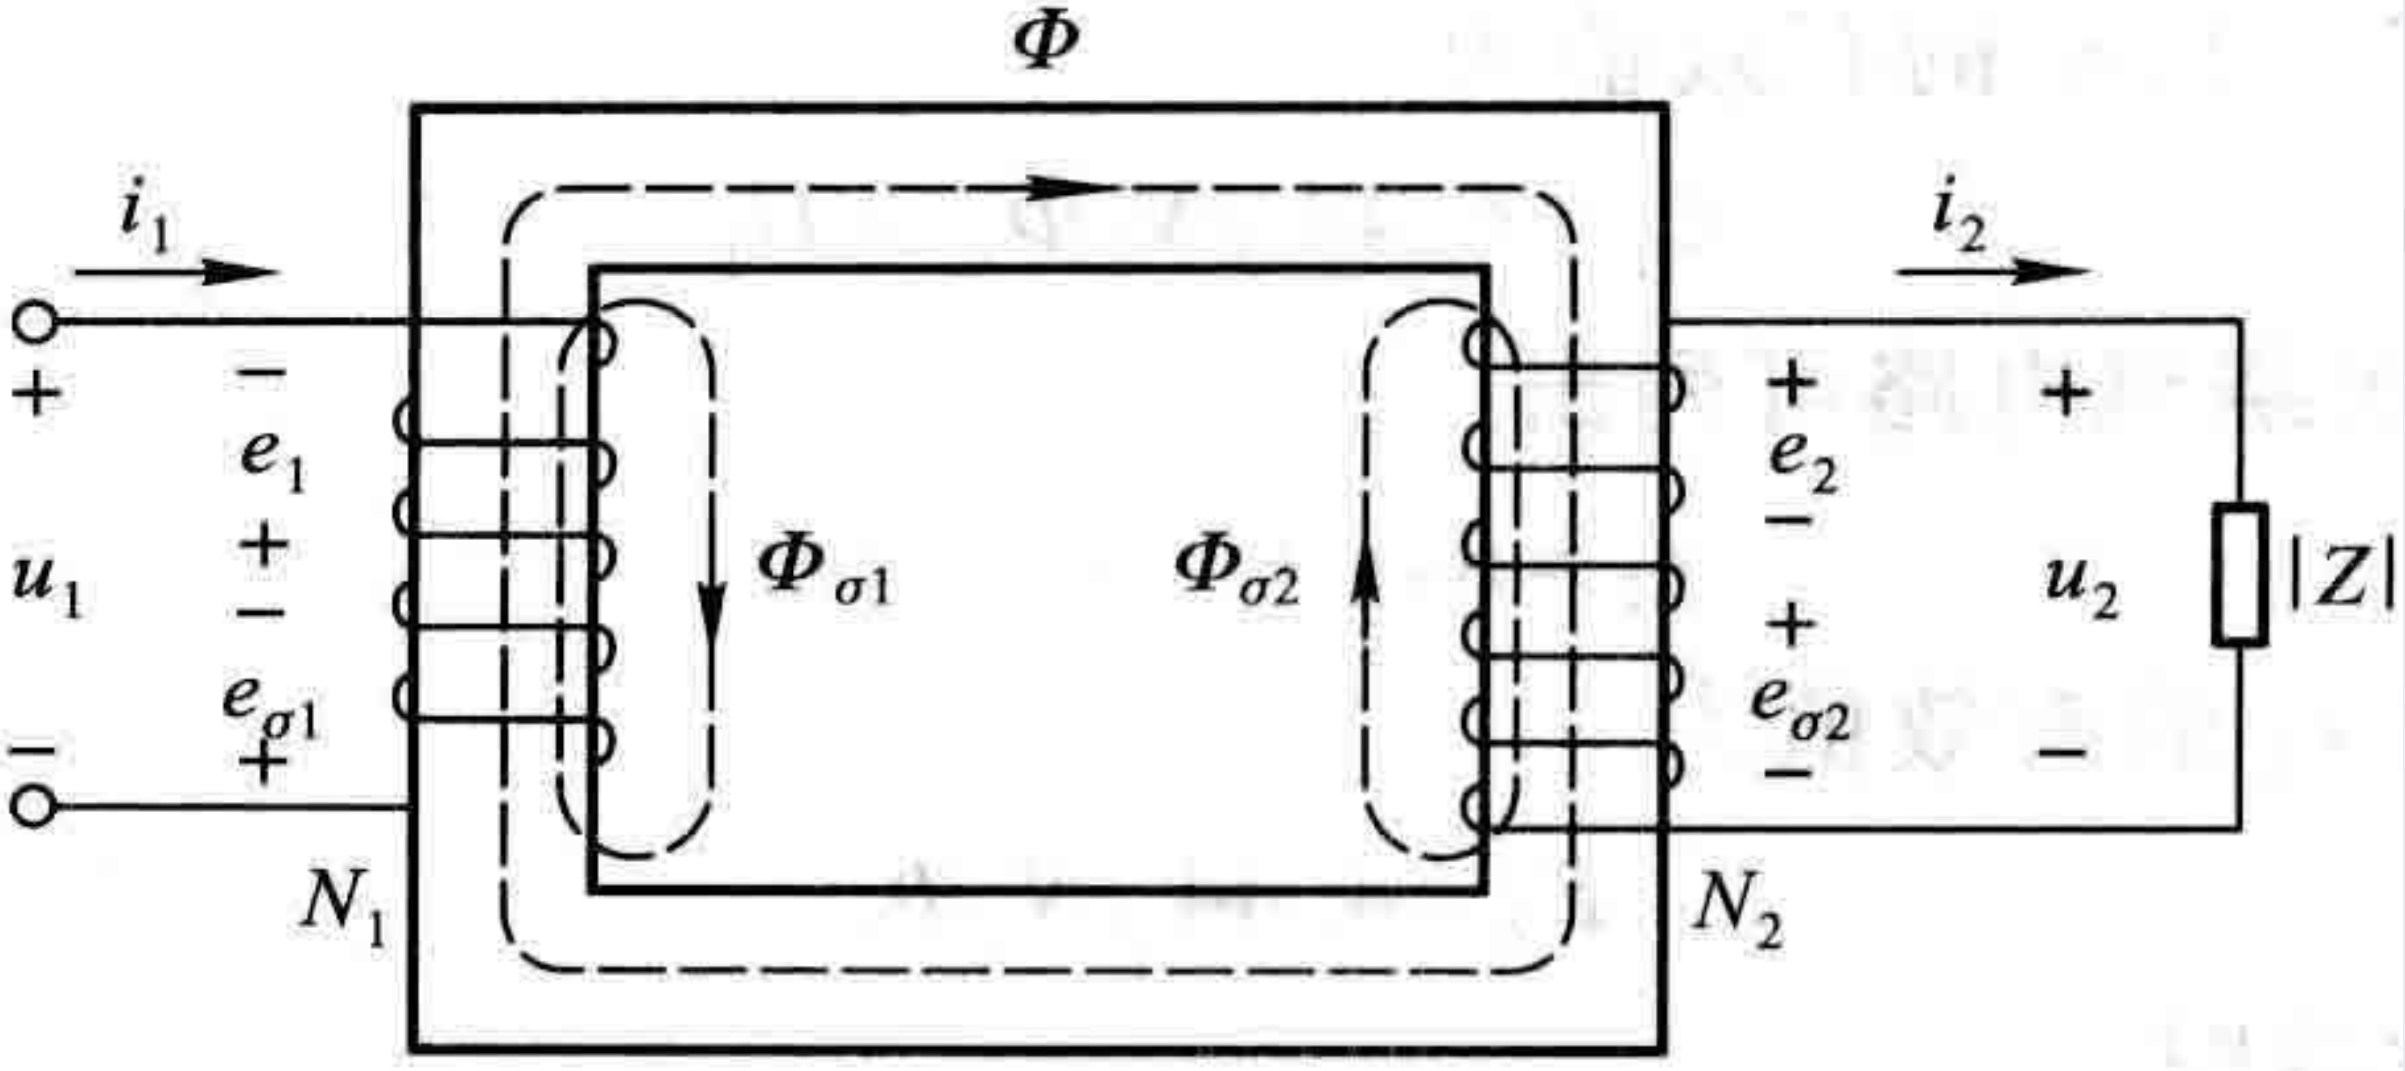
\includegraphics[width=0.65\textwidth]{变压器原理图.png}
	\caption{变压器原理图}
	\label{fig:变压器原理图}
\end{figure}

\Par 当一次绕组通上交流电$u_1$后,一次绕组中会有一个电流$i_1$,从而产生一个磁场$\boldsymbol{B}_1$,其磁通量为$\varPhi _1$,它被分成了两个部分:$\varPhi _{M1}$和$\varPhi _{\sigma 1}$.$\varPhi _{M1}$表示顺着铁芯流向了二次绕组的磁通量,它汇入了主磁通$\varPhi $,$\varPhi _{\sigma 1}$表示漏掉的磁通量.而$\varPhi $的变化在一次绕组、二次绕组上分别形成了感应电动势$e_1$、$e_2$,而二次绕组产生的磁通量也被分成了两个部分$\varPhi _{M2}$和$\varPhi _{\sigma 2}$,它们的流向同上,故而最终的流向图为
\begin{figure}[htbp]
	\centering
	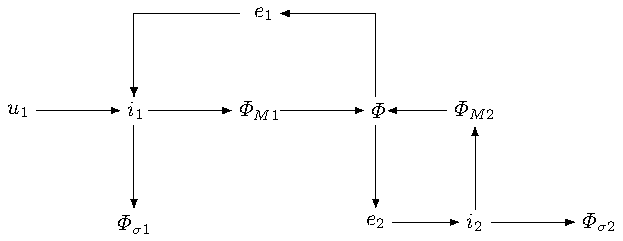
\includegraphics[width=0.65\textwidth]{变压流转图.pdf}
	\caption{变压流转图}
	\label{fig:变压流转图}
\end{figure}
\begin{enumerate}
    \item[\circledtext{1}]电压变换
    
    设主磁通$\varPhi =\varPhi _m\sin \omega t$
    \begin{equation*}
        e_1=-N\frac{\mathrm{d}\varPhi}{\mathrm{d}t}=-N\cos \omega t=2\pi fN\cdot \varPhi _m\sin \left( \omega t-\frac{\pi}{2} \right)  
    \end{equation*}
    从而有
    \begin{equation*}
        e_1=E_m\sin \left( \omega t-\frac{\pi}{2} \right) 
    \end{equation*}
    其有效值为
    \begin{equation*}
        E=\frac{E_m}{\sqrt{2}}=\sqrt{2}\pi fN\cdot \varPhi _m=4.44fN\cdot B_mS
    \end{equation*}
    根据KVL列出空载时两端电压
    \begin{equation*}
        \left\{ \begin{aligned}
            u_1&=i_0R_1+\left( -e_{\delta 1} \right) +\left( -e_1 \right) \approx -e_1\\
            u_2&=e_2\\
        \end{aligned} \right. 
    \end{equation*}
    有载时两端电压
    \begin{equation*}
        \left\{ \begin{aligned}
            u_1&=i_1R_1+\left( -e_{\delta 1} \right) +\left( -e_1 \right) \approx -e_1\\
            u_2&=e_2+e_{\delta 2}-i_2R_2\\
        \end{aligned} \right. 
    \end{equation*}
    而两种情况下它们都满足
    \begin{equation*}
        \frac{U_1}{U_2}\approx \frac{E_1}{E_2}=\frac{N_1}{N_2}=K
    \end{equation*}
    其中我们定义
    \begin{equation}
        K\coloneqq \frac{N_1}{N_2}
    \end{equation}
    称作变压器的\hl{变比}.

    \item [\circledtext{2}] 
    由磁通势平衡方程
    \begin{equation*}
        i_0N_1=i_1N_1+i_2N_2
    \end{equation*}
    近似将$i_0N_1\approx 0$可以得到
    \begin{equation*}
        \frac{i_1}{i_2}\approx -\frac{N_2}{N_1}\Longrightarrow \frac{I_1}{I_2}\approx \frac{N_2}{N_1}=\frac{1}{K}
    \end{equation*}
    \item [\circledtext{3}]
    根据
    \begin{equation*}
        \left| Z \right|=\frac{U}{I}
    \end{equation*}
    我们可以得到
    \begin{equation*}
        \frac{\left| Z_1 \right|}{\left| Z_2 \right|}\approx \frac{U_1/I_1}{U_2/I_2}=\frac{K}{\frac{1}{K}}=K^2
    \end{equation*}
\end{enumerate}
\Par 好了,变压器结束了.